\problemname{K.O. Kids}

On his birthday party, Glen wants to play the most exciting game. It
is called \emph{Splash Game}. For this, his parents built a bridge, which goes
over the full length of the family pool and can be seen as a $2 \times
n$ grid: it consists of $n$ steps and at each step, there are two
plates. The players go over the bridge one after the other in a fixed
order. At each of the $n$ steps, one of the two plates is fake and
the player will fall into the pool with a big \emph{Splaaaaash} when
she steps onto it.

Of course, a participant can be lucky and guess the real plate and
will not fall (she might still fall later). Also the first
player really has a tough time. To make it to the other side, she would
need to guess the real plate at every step. The later players have
the advantage that they can see
what the others are doing and hence know for the already entered
steps, which plate is the real one (if a player guesses the real
plate, everybody sees it; if she guesses the fake one and falls, everybody knows
that the other plate is the real one).

The players proceed by a simple strategy. The first player
starts by choosing the left plate on the first step. If she is correct,
she switches to the right side and she will keep switching the side at
every step (it is common knowledge that switching is a good
idea). Every other player, once it is her turn, follows
the correct choices as far as they are known and, afterwards, applies
the switching strategy as well, i.\,e., if she stepped on the left
plate on the previous step, she now steps on the right one and vice versa.

Of course, the game is only fun if at least a few kids make it to the
other side of the bridge. But it shouldn't be too many either, since everybody
has a great laugh when somebody is falling into the water. Given the
number of kids and the planned layout of fake and real plates,
output how many kids make it to the other side of the bridge.

\begin{figure}[ht!]
\centering
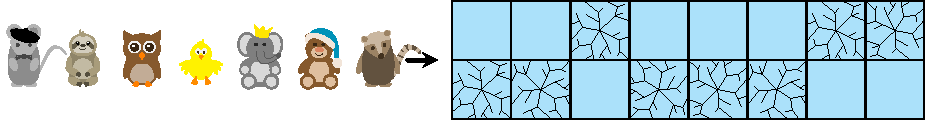
\includegraphics[width=0.9\textwidth]{sample}

\caption{The bridge layout for Sample Input 4 (cracked squares indicate
  the fake plates). The first player will
  guess the first step correctly, but fall on the second step. The
  second player thus knows the correct choices for the first two steps
  and guesses the third and fourth one correctly by switching. In the
  end, three of the seven kids make it to the other side.}
\end{figure}


\begin{Input}
	The input consists of:
  \begin{itemize}
    \item One line with integers $n, k$ ($1 \leq n,k \leq 10^3$), the
	length of the bridge and the number of kids.
    \item One string $s$ of length $n$ consisting of characters \texttt{L} and \texttt{R}. An \texttt{L} on position $i$ indicates that the real plate at step $i$ is the left one, an \texttt{R} indicates the right plate is the real one.
  \end{itemize}
\end{Input}

\begin{Output}
        Output a single integer, the number of kids who make it to the
        other side of the bridge.
\end{Output}
